\documentclass[border=10pt]{standalone}
\usepackage[svgnames]{xcolor}
\usepackage{amsmath}
\usepackage{pgfplots}
\pgfplotsset{compat=newest}
\usepackage[sfdefault]{FiraSans}
\usepackage{FiraMono}
\renewcommand*\familydefault{\sfdefault}
\begin{document}
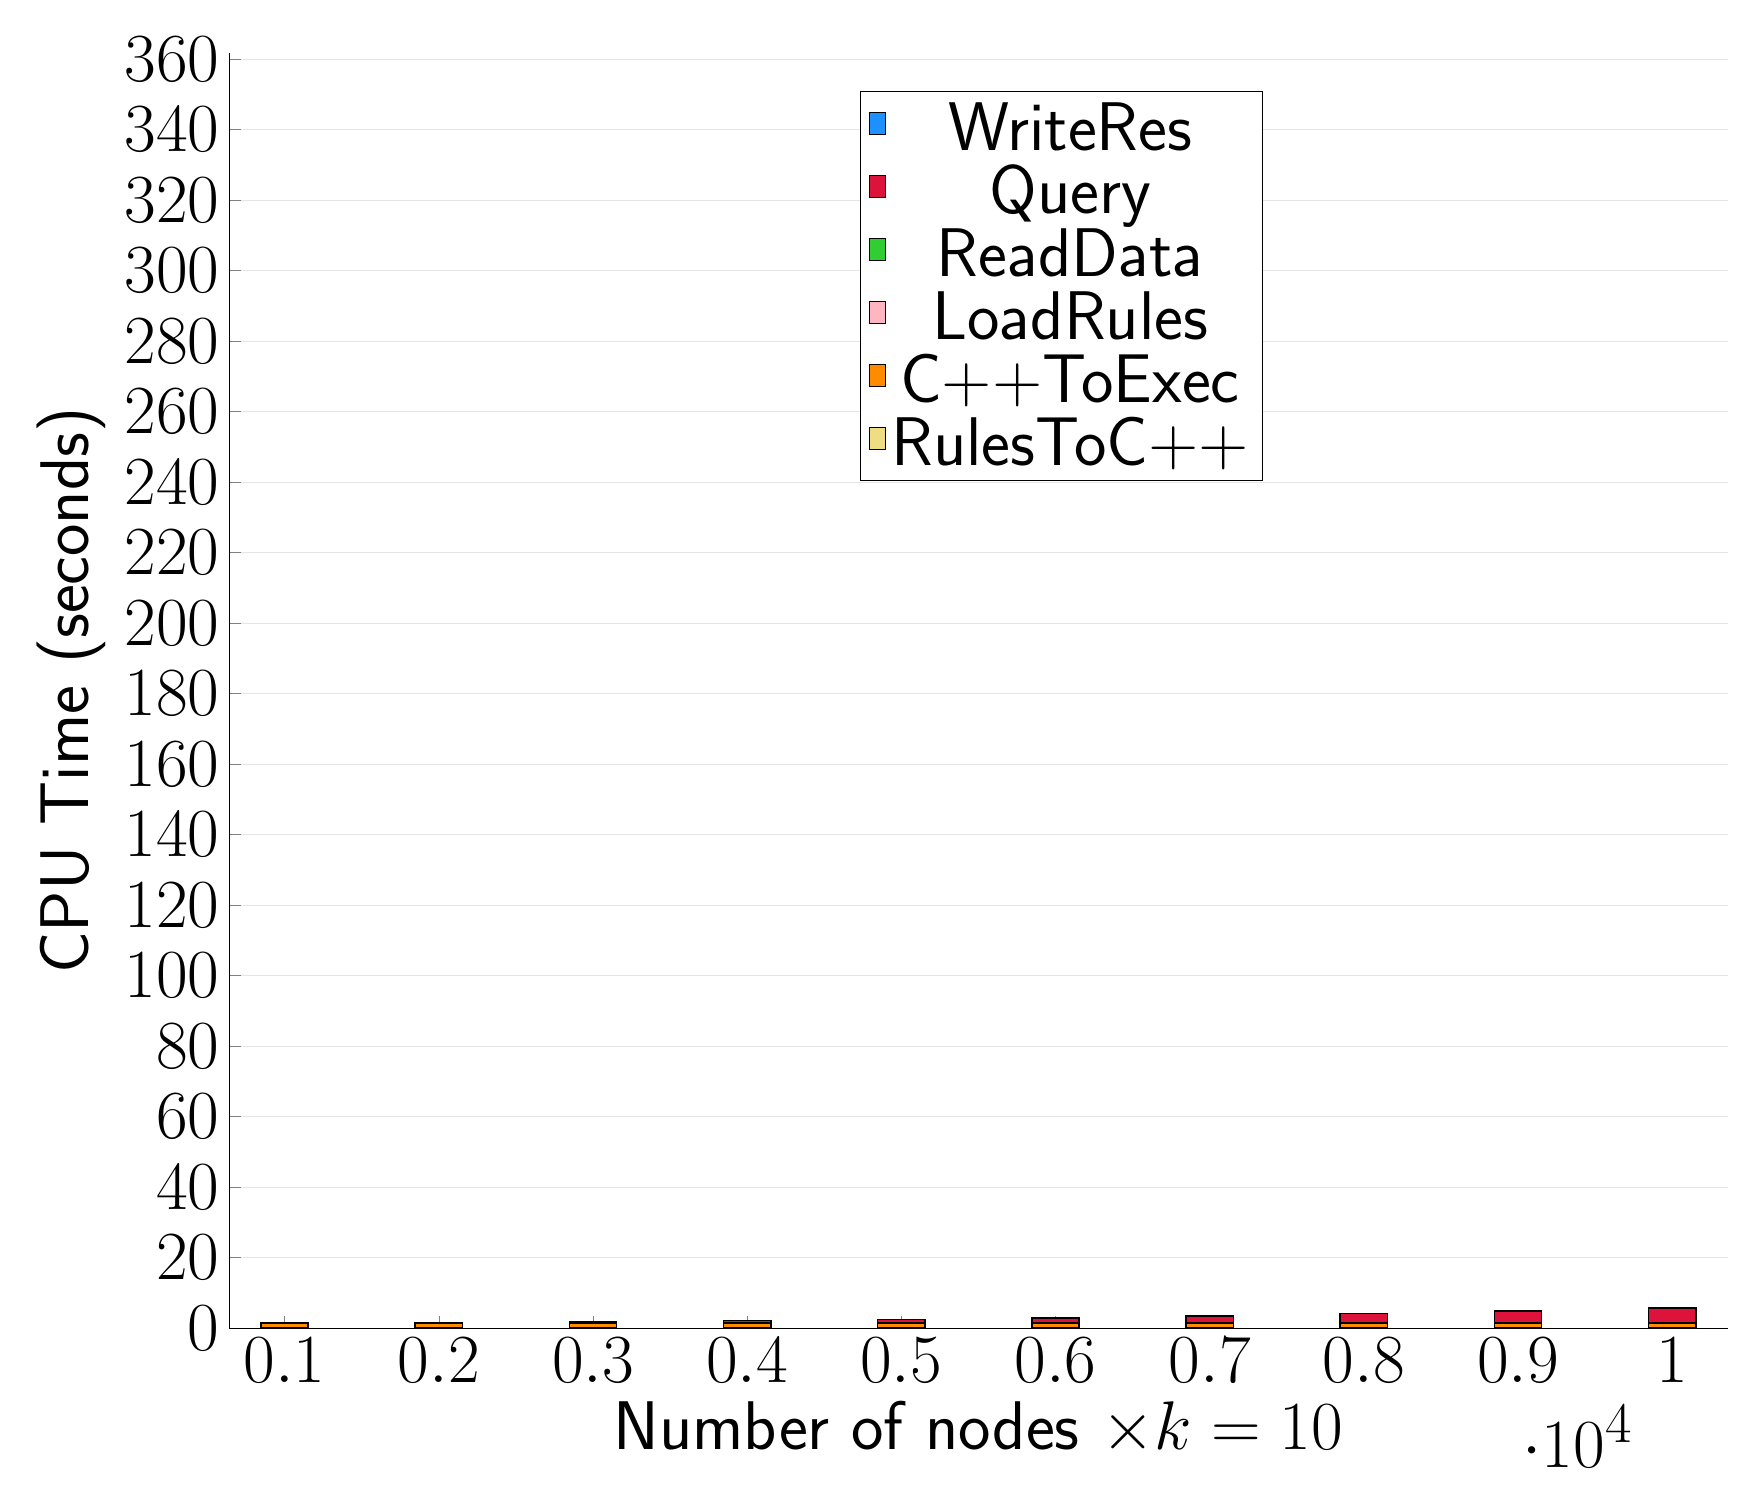
\begin{tikzpicture}
\begin{axis}[
   ybar stacked,
   width=1.7\textwidth,
   bar width=0.6cm,
   ymajorgrids, tick align=inside,
   major grid style={draw=gray!20},
   xtick=data,
   ymin=0, ymax=361.7732,
   axis x line*=bottom,
   axis y line*=left,
   enlarge x limits=0.04,
   legend style={
       at={(0.69, 0.97)},
       anchor=north east,
       legend columns=1,
       font=\Huge,
   },
   ylabel={CPU Time (seconds)},
   xlabel={Number of nodes $\times k=10$},
   label style={font=\Huge},
   tick label style={font=\Huge},
]
\addlegendimage{fill=DodgerBlue, draw=black, line width=0.2pt}
\addlegendentry{WriteRes}
\addlegendimage{fill=Crimson, draw=black, line width=0.2pt}
\addlegendentry{Query}
\addlegendimage{fill=LimeGreen, draw=black, line width=0.2pt}
\addlegendentry{ReadData}
\addlegendimage{fill=LightPink, draw=black, line width=0.2pt}
\addlegendentry{LoadRules}
\addlegendimage{fill=DarkOrange, draw=black, line width=0.2pt}
\addlegendentry{C++ToExec}
\addlegendimage{fill=LightGoldenrod, draw=black, line width=0.2pt}
\addlegendentry{RulesToC++}
\addplot +[fill=LightGoldenrod, draw=black, line width=0.55pt] coordinates {
(1000, 0.0)
(2000, 0.004000000000000001)
(3000, 0.006000000000000001)
(4000, 0.008000000000000002)
(5000, 0.006000000000000001)
(6000, 0.011999999999999999)
(7000, 0.006000000000000001)
(8000, 0.004000000000000001)
(9000, 0.008000000000000002)
(10000, 0.004000000000000001)
};
\addplot +[fill=DarkOrange, draw=black, line width=0.55pt] coordinates {
(1000, 1.5099999999999998)
(2000, 1.514)
(3000, 1.534)
(4000, 1.526)
(5000, 1.53)
(6000, 1.5079999999999998)
(7000, 1.514)
(8000, 1.53)
(9000, 1.51)
(10000, 1.512)
};
\addplot +[fill=LightPink, draw=black, line width=0.55pt] coordinates {
(1000, 0.00015120000000000002)
(2000, 0.0001296)
(3000, 0.0001372)
(4000, 0.00012200000000000001)
(5000, 0.000106)
(6000, 0.00015139999999999997)
(7000, 0.000147)
(8000, 0.0001502)
(9000, 0.00014859999999999998)
(10000, 0.0001566)
};
\addplot +[fill=LimeGreen, draw=black, line width=0.55pt] coordinates {
(1000, 0.0042788)
(2000, 0.0067758)
(3000, 0.0097442)
(4000, 0.0112322)
(5000, 0.0142844)
(6000, 0.0184228)
(7000, 0.021071)
(8000, 0.021573000000000002)
(9000, 0.0250844)
(10000, 0.026306200000000002)
};
\addplot +[fill=Crimson, draw=black, line width=0.55pt] coordinates {
(1000, 0.048771999999999996)
(2000, 0.1507262)
(3000, 0.3372654)
(4000, 0.6163836)
(5000, 0.9648374000000001)
(6000, 1.3991159999999998)
(7000, 1.9270580000000002)
(8000, 2.565728)
(9000, 3.398012)
(10000, 4.258072)
};
\addplot +[fill=DodgerBlue, draw=black, line width=0.55pt] coordinates {
(1000, 0.000226)
(2000, 0.00027860000000000005)
(3000, 0.00030599999999999996)
(4000, 0.0003398)
(5000, 0.0003132)
(6000, 0.00039820000000000003)
(7000, 0.0003842)
(8000, 0.0003522)
(9000, 0.000358)
(10000, 0.00037280000000000006)
};
\end{axis}
\end{tikzpicture}

\end{document}
